% mnras_guide.tex
%
% MNRAS LaTeX user guide
%
% v3.1 released 11 June 2020
%
% v3.0 released 22 May 2015
% (version numbers match those of mnras.cls)
%
% Copyright (C) Royal Astronomical Society 2015
% Authors:
% Keith T. Smith (Royal Astronomical Society)

% Change log
%
% v3.0   September 2013 - May 2015
%    First version: complete rewrite of the user guide
%    Basic structure taken from mnras_template.tex by the same author

%%%%%%%%%%%%%%%%%%%%%%%%%%%%%%%%%%%%%%%%%%%%%%%%%%
% Basic setup. Most papers should leave these options alone.
\documentclass[fleqn,usenatbib,useAMS]{mnras}

%%%%% AUTHORS - PLACE YOUR OWN PACKAGES HERE %%%%%

% Only include extra packages if you really need them. Common packages are:
\usepackage{graphicx}	% Including figure files
\usepackage{amsmath}	% Advanced maths commands
\usepackage{amssymb}	% Extra maths symbols
\usepackage{multicol}        % Multi-column entries in tables
\usepackage{bm}		% Bold maths symbols, including upright Greek
\usepackage{pdflscape}	% Landscape pages

%%%%%%%%%%%%%%%%%%%%%%%%%%%%%%%%%%%%%%%%%%%%%%%%%%

%%%%%% AUTHORS - PLACE YOUR OWN MACROS HERE %%%%%%
\usepackage{subcaption}
% Please keep new commands to a minimum, and use \newcommand not \def to avoid
% overwriting existing commands. Example:
%\newcommand{\pcm}{\,cm$^{-2}$}	% per cm-squared
\newcommand{\kms}{\,km\,s$^{-1}$} % kilometres per second
\newcommand{\bibtex}{\textsc{Bib}\!\TeX} % bibtex. Not quite the correct typesetting, but close enough

%%%%%%%%%%%%%%%%%%%%%%%%%%%%%%%%%%%%%%%%%%%%%%%%%%


% Use vector fonts, so it zooms properly in on-screen viewing software
% Don't change these lines unless you know what you are doing
\usepackage[T1]{fontenc}
\usepackage{ae,aecompl}

% MNRAS is set in Times font. If you don't have this installed (most LaTeX
% installations will be fine) or prefer the old Computer Modern fonts, comment
% out the following line
\usepackage{newtxtext,newtxmath}
% Depending on your LaTeX fonts installation, you might get better results with one of these:
%\usepackage{mathptmx}
%\usepackage{txfonts}

%%%%%%%%%%%%%%%%%%% TITLE PAGE %%%%%%%%%%%%%%%%%%%

% Title of the paper, and the short title which is used in the headers.
% Keep the title short and informative.
	\title[Kalman PTA]{State-space PTA}

% The list of authors, and the short list which is used in the headers.
% If you need two or more lines of authors, add an extra line using \newauthor
\author[Kimpson]{Kimpson$^{1}$, Melatos, O'Leary, Evans, others, etc. etc. %
\thanks{Contact e-mail: \href{mailto:mn@ras.ac.uk}{mn@ras.ac.uk}}%
\thanks{Present address: Science magazine, AAAS Science International, \mbox{82-88}~Hills Road, Cambridge CB2~1LQ, UK}%
\\
% List of institutions
$^{1}$Royal Astronomical Society, Burlington House, Piccadilly, London W1J 0BQ, UK}

% These dates will be filled out by the publisher
\date{Last updated 2020 June 10; in original form 2013 September 5}

% Enter the current year, for the copyright statements etc.
\pubyear{2020}

% Don't change these lines
\begin{document}
\label{firstpage}
\pagerange{\pageref{firstpage}--\pageref{lastpage}}
\maketitle

% Abstract of the paper
\begin{abstract}
This is an abstract
\end{abstract}

% Select between one and six entries from the list of approved keywords.
% Don't make up new ones.
\begin{keywords}
editorials, notices -- miscellaneous
\end{keywords}

%%%%%%%%%%%%%%%%%%%%%%%%%%%%%%%%%%%%%%%%%%%%%%%%%%

%%%%%%%%%%%%%%%%% BODY OF PAPER %%%%%%%%%%%%%%%%%%

% The MNRAS class isn't designed to include a table of contents, but for this document one is useful.
% I therefore have to do some kludging to make it work without masses of blank space.
\begingroup
\let\clearpage\relax
%\tableofcontents
\endgroup
\newpage

\section{Introduction}



The detection of high frequency ($\sim1$ Hz) gravitational waves (GWs) from coalescing black hole (BH) binaries with ground-based detectors such as LIGO/Virgo \citep{aLIGO,2015CQGra..32b4001A} is now a routine enterprise \citep[e.g.][]{2019PhRvX...9c1040A,2021PhRvX..11b1053A}. Gravitational radiation from sources which radiate in the mill-Hz regime are expected to be detectable from $\sim 2037$ with the space-based Laser Interferometer Space Antenna, \citep{LISApaper}, especially given the early success by the pathfinder mission \citep{2019arXiv190308924A}. Detecting GWs from systems which evolve over even longer timescales, $\mathcal{O}$(years), has necessitated the development of novel astrophysical methods, since it is practically impossible to engineer interferometric detectors with sufficiently long baselines. The foremost technique for the detection of GWs in this nano-Hz regime is a via timing an ensemble of milliseconds pulsars; a pulsar timing array (PTA) \citep{2021hgwa.bookE...4V}. The presence  of a nano-Hz gravitational wave will influence the propagation of the pulsar radio beacon, leaving a characteristic impression on the pulsar timing signal. By measuring the modulation of the received pulsar signal in this way, one can effectively construct a detector with a baseline on the scale of parsecs. \newline 


\noindent Multiple PTA detectors have now been built over the last few decades, including the North American Nanohertz Observatory for Gravitational Waves \citep[NANOGrav,][]{2020ApJ...905L..34A}, the Parkes Pulsar Timing array \citep[PPTA][]{2020PASA...37...20K}, and the European Pulsar Timing Array \citep[EPTA,][]{2010CQGra..27h4014F}. These previously disparate efforts have now been joined in international collaboration, along with a number of newer PTAs such as the Indian Pulsar Timing Array Project \citep[InPTA,][]{ipta}, under the umbrella of the International Pulsar Timing Array \citep[IPTA][]{2019MNRAS.490.4666P}. The primary target of PTA observations is the gravitational radiation emitted from the inspiral of supermassive black hole binaries (SMBHBs) with masses $\sim 10^7 M_{\odot}$. These GW signals from SMBHBs can be broadly classified into either deterministic or stochastic. For the former, sufficiently bright and near binaries may be resolvable with PTAs, allowing the very earliest stages of their evolution and coalescence to be investigated \citep{Zhu10}. For the latter, the incoherent superposition of multiple weaker SMBHBs sources leads to a stochastic background detectable at nano-Hz frequencies \citep{Sesana10}. Other potential sources for PTAs include cosmic strings \citep[e.g.][]{PTAstring} and cosmological phase transitions \citep[e.g.][]{PTAphase}, but the deterministic and stochastic GW signals from SMBHBs remain the primary targets. \newline 

\noindent The detection of loud, resolved sources with a PTA typically involves a parametrised model for the pulsar timing residuals induced by the modulation of the pulsar signal by a GW. One can then search for evidence that this model describes the data via the usual Bayesian likelihood techniques, and try to estimate the parameters of the model \citep[e.g.][]{Babak2016}. For detecting the stochastic background the approach is different; one measures the correlation in pulsar timing residuals between any two pair of pulsars. The presence of a GW induces a characteristic correlation function as a function of the angular separation between the pulsars; the Hellings-Downs curve \citep{Hellings}. For both classes of source, the detection of GW signals in the timing residuals of a PTA is a challenging enterprise, and currently neither a stochastic background nor an individually resolved source has yet been detected \citep{2022MNRAS.510.4873A, 10.1093/nsr/nwx126}. \newline 




\noindent The sensitivity of a PTA to a GW signal is heavily dependent on the total level of noise in the array \citep{Wang2015}. In particular, the intrinsic pulsar timing noise - i.e.  random variations in the pulse arrival time - has been identified as a key factor limiting the sensitivity of PTAs to GW signals \citep{Shannon2010,Lasky2015,Caballero2016}. This pulsar timing noise has multiple potential theorized causes including microglitches \citep{Melatos2008}, glitch recovery \citep{Hobbs2010glitch}, fluctuations in both the internal and external stochastic torques \citep{Antonelli2023} and superfluid turbulence \citep{Melatos2014}. In order to mitigate the influence of timing noise, PTAs are typically composed of millisecond pulsars (MSPs) which are known to be much more stable rotators with minimal timing noise. However, timing noise in MSPs could be a `latent' phenomenon \citep{Shannon2010}; as we increase the length of observation spans and the measurement timing precision to the levels required to detect gravitational waves, the timing noise in MSPs may emerge and become much more apparent, visible in the same way that timing noise is seen in younger pulsars. In addition to timing noise there are also secondary noise sources that must be considered such as phase jitter noise and radiometer noise \citep{Cordes2010,Lam2019,Parthasarathy2021}. \newline 


\noindent In the standard approach to PTA-GW analysis, timing noise is a nuisance which must be accurately modelled and subtracted. It fundamentally limits the sensitivity of the PTA detector to a GW signal, and the ability of an observer to infer the GW source parameters. Motivated by these challenges faced by the classic PTA analysis methods, in this work we present a novel approach to formulate PTA analysis and GW detection as a state-space problem. This approach enables the pulsar state-space evolution to be tracked optimally, given a specific realisation of the pulsar process noise (i.e. the spin wandering of the pulsar), and determine both the presence of a GW signal in the pulsar data, and  infer the underlying source parameters. For this initial exploratory study we will focus exclusively on resolved, monochromatic GW sources. \textcolor{red}{TK: This motivation section is weak. Need to think about how to phrase this better. Be clear on the real challenges of the "old" approach and the advantages of the "new" one.} \newline 


\noindent This paper is organised as follows:  \textcolor{red}{TK: TBD} \newline 


\noindent We adopt the natural units, with $c = G = \hbar = 1$, and a
$(-,+,+,+)$ metric signature. \newline 



\section{State-Space Model}
We want to formulate the PTA analysis as a state-space problem with a separation between the intrinsic pulsar state, $\bar{x}$, and the measurement state recorded by an observer,$\bar{y}$. We will take our state variable to be the intrinsic pulsar pulse frequency $f(t)$, as measured in the momentarily comoving reference frame of an observer local to the pulsar. We will now consider how the intrinsic pulse frequency evolves in time, completely separate from the influence of a GW, and then go on to derive the  influence of a GW perturbation on the frequency recorded by an observer at Earth. \textcolor{red}{Need some extra discussion here on why this choice of state/measurement space. Why not e.g. phase, TOA, voltage, etc. ?}

\subsection{Evolution of the pulsar frequency}
We will take as our model of the intrinsic pulsar frequency $f$ a variation of the phenomenological model of \cite{Vargas}. Within this model, $f$ evolves according to a combination of both deterministic torques (i.e. electromagnetic spin-down) and stochastic torques (i.e. `spin wandering', achromatic variations in the pulse TOA intrinsic to the star). The deterministic torque is taken to arise from the pulsar magnetic dipole, with braking index $n=3$ whilst the stochastic torque is a simple white noise process. Specifically, the frequency evolves according to a Ornstein-Uhlenbeck process (equivalently a Langevin equation) with a time-dependent drift parameter:
\begin{equation}
	\frac{df}{dt} = -\gamma	 [f - f_{\rm EM} (t)] + \dot{f}_{\rm EM} + \xi(t)
	\label{eq:frequency_evolution}
\end{equation}
where $f_{\rm EM}$ is the solution of the electromagnetic spindown equation,$\dot{f}_{\rm EM}$ is the spin derivative, $\gamma$ a proportionality constant that specifies the mean-reversion timescale, and $\xi(t)$ a white noise process that satisfies,
\begin{equation}
	\langle \xi(t) \xi(t') \rangle = \sigma^2 \delta(t - t')
\end{equation}
for variance $\sigma^2$. For PTA analysis, we are concerned with timescales on the order of years. Consequently, we can express the EM spindown straightforwardly as
\begin{equation}
	f_{\rm EM} (t) = f_{\rm EM}(0) + \dot{f}_{\rm EM} (0)t
\end{equation}  
Completely, the frequency evolution is then given by the solution of the stochastic differential equation,
\begin{equation}
	\frac{df}{dt} = -\gamma	 [f - f_{\rm EM}(0) - \dot{f}_{\rm EM} (0)t] + \dot{f}_{\rm EM} (0) + \xi(t)
	\label{eq:frequency_evolution_expanded}
\end{equation}
As emphasised in \cite{Vargas}, this model for the frequency evolution is a phenomenological model that aims to qualitatively reproduce the typical behaviour of observed pulsars, rather than being derived from a physical model of the neutron star \citep[e.g. a model of the neutron star crust and superfluid, components][]{Meyers2021}. For our purposes of exploring the detection of GWs via a state space formulation it will prove sufficiently accurate and appropriate.

\subsection{Modulation of pulsar frequency due to a GW}
In the presence of a GW, the $f(t)$  measured by an observer in the local NS reference frame is different from that measured by an observer on Earth. We want to determine quantitatively determine this difference - how the GW influences the received pulse frequency.

\subsubsection{Plane GW perturbation}
We take a gravitational plane wave that perturbs a background Minkowski spacetime as
\begin{equation}
	g_{\mu \nu} = \eta_{\mu \nu} + H_{\mu \nu} e^{i(\Omega(\bar{n} \cdot \bar{x} - t) + \Phi_0)	}
\end{equation}
for Minkowski metric $ \eta_{\mu \nu}$, spatial coordinates $\bar{x}$, \textcolor{red}{(TK: We have a notation conflict between $x$ = state and $x$ = coordinates)} where the GW has a constant angular frequency $\Omega$, propagates in the $\bar{n}$-direction and has a phase offset of  $\Phi_0$. We emphasise that $\Omega$ has no time dependence - we are concerned solely with monochromatic sources. Note that we are free to choose our coordinate system such that $\Phi_0$ is the GW phase at $t=0$ \textit{at the Earth.}\footnote{\textcolor{red}{TK: This point is important, since the phase offset is then the same between multiple pulsars. See also Melatos 2022 PT12}}. The amplitude tensor $H_{\mu \nu}$ has zero temporal components ($H_{0 \mu} = H_{\mu 0} = 0$) whilst the spatial part is
\begin{align}
	H_{ij} = h_+ e_{ij}^+(\bar{n}) + h_{\times} e_{ij}^{\times}(\bar{n})
\end{align}
where  $h_{+,\times}$ are the polarisation amplitudes of the gravitational plane wave. The polarisation tensors $e_{ij}^{+,\times}$ are uniquely defined by the principal axes of the wave:
\begin{align}
	e_{a b}^{+}(\hat{\Omega}) =\hat{m}_a \hat{m}_b-\hat{n}_a \hat{n}_b \\
		e_{a b}^{\times}(\hat{\Omega}) =\hat{m}_a \hat{n}_b+\hat{n}_a \hat{m}_b
\end{align}
which are in turn specified via the location of the GW source on the sky (via $\theta$, $\phi$ coordinates) and the polarisation angle $\psi$
\begin{align}
	\vec{m} & =(\sin \phi \cos \psi-\sin \psi \cos \phi \cos \theta) \hat{x} \nonumber \\
	& -(\cos \phi \cos \psi+\sin \psi \sin \phi \cos \theta) \hat{y} \nonumber \\
	& +(\sin \psi \sin \theta) \hat{z} \\
	\vec{n} & =(-\sin \phi \sin \psi-\cos \psi \cos \phi \cos \theta) \hat{x} \nonumber \\
	& +(\cos \phi \sin \psi-\cos \psi \sin \phi \cos \theta) \hat{y}\nonumber  \\
	& +(\cos \psi \sin \theta) \hat{z}
\end{align}

\subsubsection{Pulse frequency as a photon}
\noindent We will consider the pulse frequency as a photon with covariant 4-momentum $p_{\mu}$. Generally, the frequency of a photon recorded by an observer with 4-velocity $u^{\mu}$ is 
\begin{equation}
	\nu = p_{\alpha} u^{\alpha}
\end{equation}
\noindent We consider both our emitter and receiver to be stationary, such that  
\begin{equation}
	u^{\alpha}|_{\rm emitter} = u^{\alpha}|_{\rm receiver} = (1,0,0,0)
\end{equation}
\noindent Consequently the frequency can be directly identified with the temporal component of the covariant 4-momentum,
\begin{equation}
	f = p_t
\end{equation}
\noindent The expression for the evolution of the pulse frequency as measured by the observer on Earth is then,
\begin{equation}
	p_t(t_1)|_{\rm Earth} = p_t(t_0)|_{\rm source} + \int_{t = t_0}^{t=t_1} \dot{p}_t dt
\end{equation}
\noindent where the overdot denotes a derivative w.r.t. $t$. Since the influence of the GW perturbation on $\dot{p}_t$ is small, we can relate the source emission and receiver times as $t_1 = t_0 + d$ and consider the photon trajectory to be an unperturbed path. \footnote{\textcolor{red}{TK: See also e.g. Maggiore, Meltaos who takes the same approach...}} \newline 

\noindent To complete our expression, we now just need to determine $\dot{p}_t$ and integrate it.

\subsubsection{Hamiltonian Mechanics}
The Hamiltonian in covariant notation can be written as 
\begin{equation}
	H(x^{\mu}, p_{\mu}) = \frac{1}{2} g_{\mu \nu} p^{\mu} p^{\nu},
\end{equation}
\noindent which if we substitute in our expression for the perturbed metric is
\begin{equation}
	H = \frac{1}{2} \eta_{\mu \nu} p^{\mu} p^{\nu} + \frac{1}{2} H_{ij}p^i p^j e^{i(\Omega(\bar{n} \cdot \bar{x} - t) + \Phi_0)	}
\end{equation}
\noindent Now, Hamilton's equations are
\begin{equation}
	\frac{dx^{\mu}}{d\lambda} = \frac{\partial H}{\partial p_{\mu}} , \, \, \frac{dp_{\mu}}{d \lambda} = -\frac{\partial H}{\partial x^{\mu}} 
\end{equation}

\noindent for affine parameter $\lambda$. The derivative of the temporal component of the covariant momenta is then,
\begin{equation}
	\frac{d p_{t}}{d \lambda} = -\frac{i\Omega}{2} H_{ij}p^i p^j  e^{i(\Omega(\bar{n}\cdot \bar{x} - t))+\Phi_0}
\end{equation}
\footnote{\textcolor{red}{TK: This is equivalent to Melatos 2018, Eq 5 for the specific case of a GW propagating in the $z$-direction, with zero phase offset}.}


\noindent Therefore the derivative w.r.t coordinate time $t$ is,
\begin{equation}
	\dot{p}_t = \frac{d p_{t}}{d \lambda} \left(\frac{dt}{d\lambda}\right)^{-1} = \frac{d p_{t}}{d \lambda} \left(\frac{1}{p^t}\right)
\end{equation}
\noindent Note that $\dot{p}_t$ is entirely a function of the GW perturbation. In the Minkowski case the spacetime is stationary and so $p_t$ should be conserved along the geodesic. It will prove useful to recognise that $p^{\mu} = \omega(1,-q^x,-q^y,-q^z)$ where $\bar{q}$ is the unit vector between the Earth and pulsar and $\omega$ is the \textit{constant} photon angular frequency. Given the small effect of the GW perturbation, at first order we can identify $\omega$ as either the frequency at source or observer \footnote{ \textcolor{red}{TK: see Melatos 2022, PT16}}. We will consider  the pulsar locations to be constant with respect to the Earth. In practice, the pulsar locations vary with respect to the Earth, but are constant with respect to the solar system barycentre (SSB). This barycentering correction is typically applied during the pulsar detection process. Our conclusions are generally unchanged by this choice - it is straightforward to transform $q$ if needed into a vector between the SSB and pulsar. The spatial coordinates along the photon path are related to the pulsar as $\bar{x}(t) = -\bar{q}t$. \newline  


\noindent Bringing this all together we can write $\dot{p}_t$ in a condensed form as,
\begin{equation}
	\dot{p}_t = A e^{i \gamma t + \Phi_0}
\end{equation}
where 
\begin{equation}
	\gamma = -\Omega (1 + \bar{n}\cdot \bar{q}) 
\end{equation}
\footnote{\textcolor{red}{TK: compare with Melatos 2022, PT11}}
\noindent and
\begin{equation}
	A = -\frac{i\Omega \omega}{2} H_{ij}q^i q^j 
\end{equation}

\subsubsection{Performing the integral}

The frequency shift experienced by the observer relative to the source due to a GW is then
\begin{align}
	p_t(\tau)|_{\rm Earth} - p_t(\tau - d)|_{\rm source} = A \int_{t = \tau - d}^{t=\tau} e^{i \gamma t + \Phi_0}dt  \\
	=\frac{-iA}{\gamma} e^{i \gamma \tau}e^{\Phi_0}[1 - e^{-i \gamma d}] 
	\label{eq:concise}
\end{align}
We can write this more explicitly as,
\begin{align} \label{eq:final}
	&p_t(\tau)|_{\rm Earth} - p_t(\tau - d)|_{\rm source} = \\
	&\frac{ \omega}{2} \frac{H_{ij}q^i q^j  }{(1 + \hat{n} \cdot \hat{q})}e^{-i \Omega \tau(1+\bar{n} \cdot \bar{q}) + \Phi_0} [1 - e^{i \Omega(1+\bar{n} \cdot \bar{q}) d}]
\end{align}
or alternatively, with $h_{ij} = g_{ij} - \eta_{ij}$,
\begin{equation}
	p_t(\tau)|_{\rm Earth} - p_t(\tau - d)|_{\rm source} =\frac{ \omega}{2} \frac{h_{ij} q^i q^j  }{(1 + \hat{n} \cdot \hat{q})} [1 - e^{i \Omega(1+\bar{n} \cdot \bar{q}) d}]
	\label{eq:freq_shift}
\end{equation}

\subsection{State-space structure} \label{sec3}
We now have a model for the evolution of the intrinsic pulsar frequency states and the measured frequency timeseries. We can express the intrinsic frequency evolution, Eq. \ref{eq:frequency_evolution_expanded}, in a alternative form as,
\begin{equation}
	df = \mathcal{A} f dt + N(t) dt + \sigma dB(t)
	\label{eq:state1}
\end{equation}
where $\mathcal{A} = -\gamma$, $N(t) = \gamma(f_{\rm EM}(0) + \dot{f}_{\rm EM}(0) t) +\dot{f}_{\rm EM}(0)$ and $dB(t)$ denotes increments of Brownian motion (Wiener process). This equation is easily identified as an Ornstein-Uhlenbeck process which has a general solution given by \citep{gardiner2009stochastic},
\begin{equation}
	f(t) = e^{\mathcal{A}t}f(0) + \int_0^t e^{\mathcal{A}(t-t')} N(t') dt' + \int_0^t e^{\mathcal{A}(t-t')} \sigma dB(t')
\end{equation} 
If we move from a solution in continuous time to discrete time then
\begin{equation}
	f(t_{i+1}) = F f(t_i) + T_i + \eta_i
\end{equation}
where
\begin{equation}
	F_i = e^{A (t_{i+1} - t_i)}
\end{equation}
\begin{equation}
	T_i = \int_{t_i}^{t_{i+1}}  e^{A (t_{i+1} - t')} N(t') dt'
\end{equation}
\begin{equation}
	\eta_i = \int_{t_i}^{t_{i+1}}  e^{A (t_{i+1} - t')} \sigma dt'
\end{equation}
Given the discrete solution $f(\bar{t})$ where $\bar{t} = (t_1, t_2, ...,t_N)$ the intrinsic frequency can be related to the measured frequency as 
\begin{equation}
	f_M (\bar{t})= f g(\bar{\theta},\bar{t}) + N_M
\end{equation}
where $g(\theta,t)$ ("measurement function") is a function of some constant parameters, $\bar{\theta}$, and discrete time $\bar{t}$, whilst $N_M$ is a Gaussian measurement noise that satisfies 
\begin{equation}
	\langle N_M(t) N_M(t') \rangle = \Sigma^2 \delta(t - t')
\end{equation}
for variance $\Sigma^2$. The measurement function follows from Eq. \ref{eq:freq_shift}
\begin{equation} \label{eq:final}
	g(\bar{\theta},t) = 1 - \frac{1}{2} \frac{h_{ij}(t) q^i q^j}{1 + \bar{n} \cdot \bar{q}}[1 - e^{i \Omega(1+\bar{n} \cdot \bar{q}) d}]
\end{equation}
or in a more concise form where we have switched to a trigonometric form of the equations and made the time dependence explicit,
\begin{equation} 
	g(\bar{\theta},t) = 1 -A \cos(-\Omega t (1 + n\cdot q ) + \Phi_0)
\end{equation}
where 
\begin{equation}
	A =  \frac{1}{2} \frac{H_{ij} q^i q^j}{1 + \bar{n} \cdot \bar{q}}[1 - \cos\left( {\Omega(1+\bar{n} \cdot \bar{q}) d}\right)]
		\label{eq:state2}
\end{equation}


\section{Detection and parameter estimation}
Let's  review and categorise all the parameters of above state-space model. We can generally separate these into parameters which correspond to the intrinsic frequency evolution of the pulsar, the GW parameters and the noise parameters i.e.
\begin{equation}
	\bar{\theta} =  \bar{\theta}_{\rm PSR} \cup \bar{\theta}_{\rm GW} \cup \bar{\theta}_{\rm noise}
\end{equation}
\begin{equation}
	\bar{\theta}_{\rm PSR} = [\gamma, f_{\rm EM}(0), \dot{f}_{\rm EM}(0),d]^{(N)}
\end{equation}
\begin{equation}
	\bar{\theta}_{\rm GW} = [h_{+}, h_{\times}, \delta, \alpha, \psi, \Omega, \Phi_0]
\end{equation}
\begin{equation}
	\bar{\theta}_{\rm noise} = [\sigma, \Sigma]
\end{equation}
\textcolor{red}{TK: $\sigma$ is currently a parameter shared between all pulsars in current code implementation. Probably need to update this since different pulsars have different process noise, but need to check identifiability and likelihood curves - only enters the Kalman filter only through the process noise matrix...}. Whilst the GW parameters are shared between measurements for each pulsar, the pulsar parameters are clearly not. For a PTA dataset of $N$ pulsars we have $7 + 5N$ parameters to estimate. For now we will consider the measurement noise to be known, although in principle this too could be estimated. Note that whilst this is a large parameter space, in general the pulsar parameters are much better constrained than the GW parameters: for example we have rough estimates for the pulsar distances accurate to $\sim$ 10$\%$, but we have no prior information on the source location. \newline 

\noindent We want be able to infer the values of the model parameters and look for evidence of a GW signal in a data stream. To this end, we will use a Kalman filter in to obtain likelihood estimates of the data given a set of parameters. We will then deploy the Kalman filter in conjunction with a nested sampling technique for optimisation of the parameters over the likelihood. We will now review the Kalman filter and the associated likelihood in Section \ref{sec:kalman_filter} before going on in Section \ref{sec:nested_sampling} to discuss how to use nested sampling methods together with the filter for detection (model selection) and parameter estimation. We go on to discuss our choice of pulsars to make up our PTA in Section \ref{sec:pta_pulsars}, before deploying these techniques in Sections \ref{sec:param_estimation} , \ref{sec:detection} for parameter estimation and model selection.

\subsection{Kalman Filtering}\label{sec:kalman_filter}
\begin{figure*}
	%\centering % Not needed
	\begin{subfigure}[b]{1\columnwidth}
		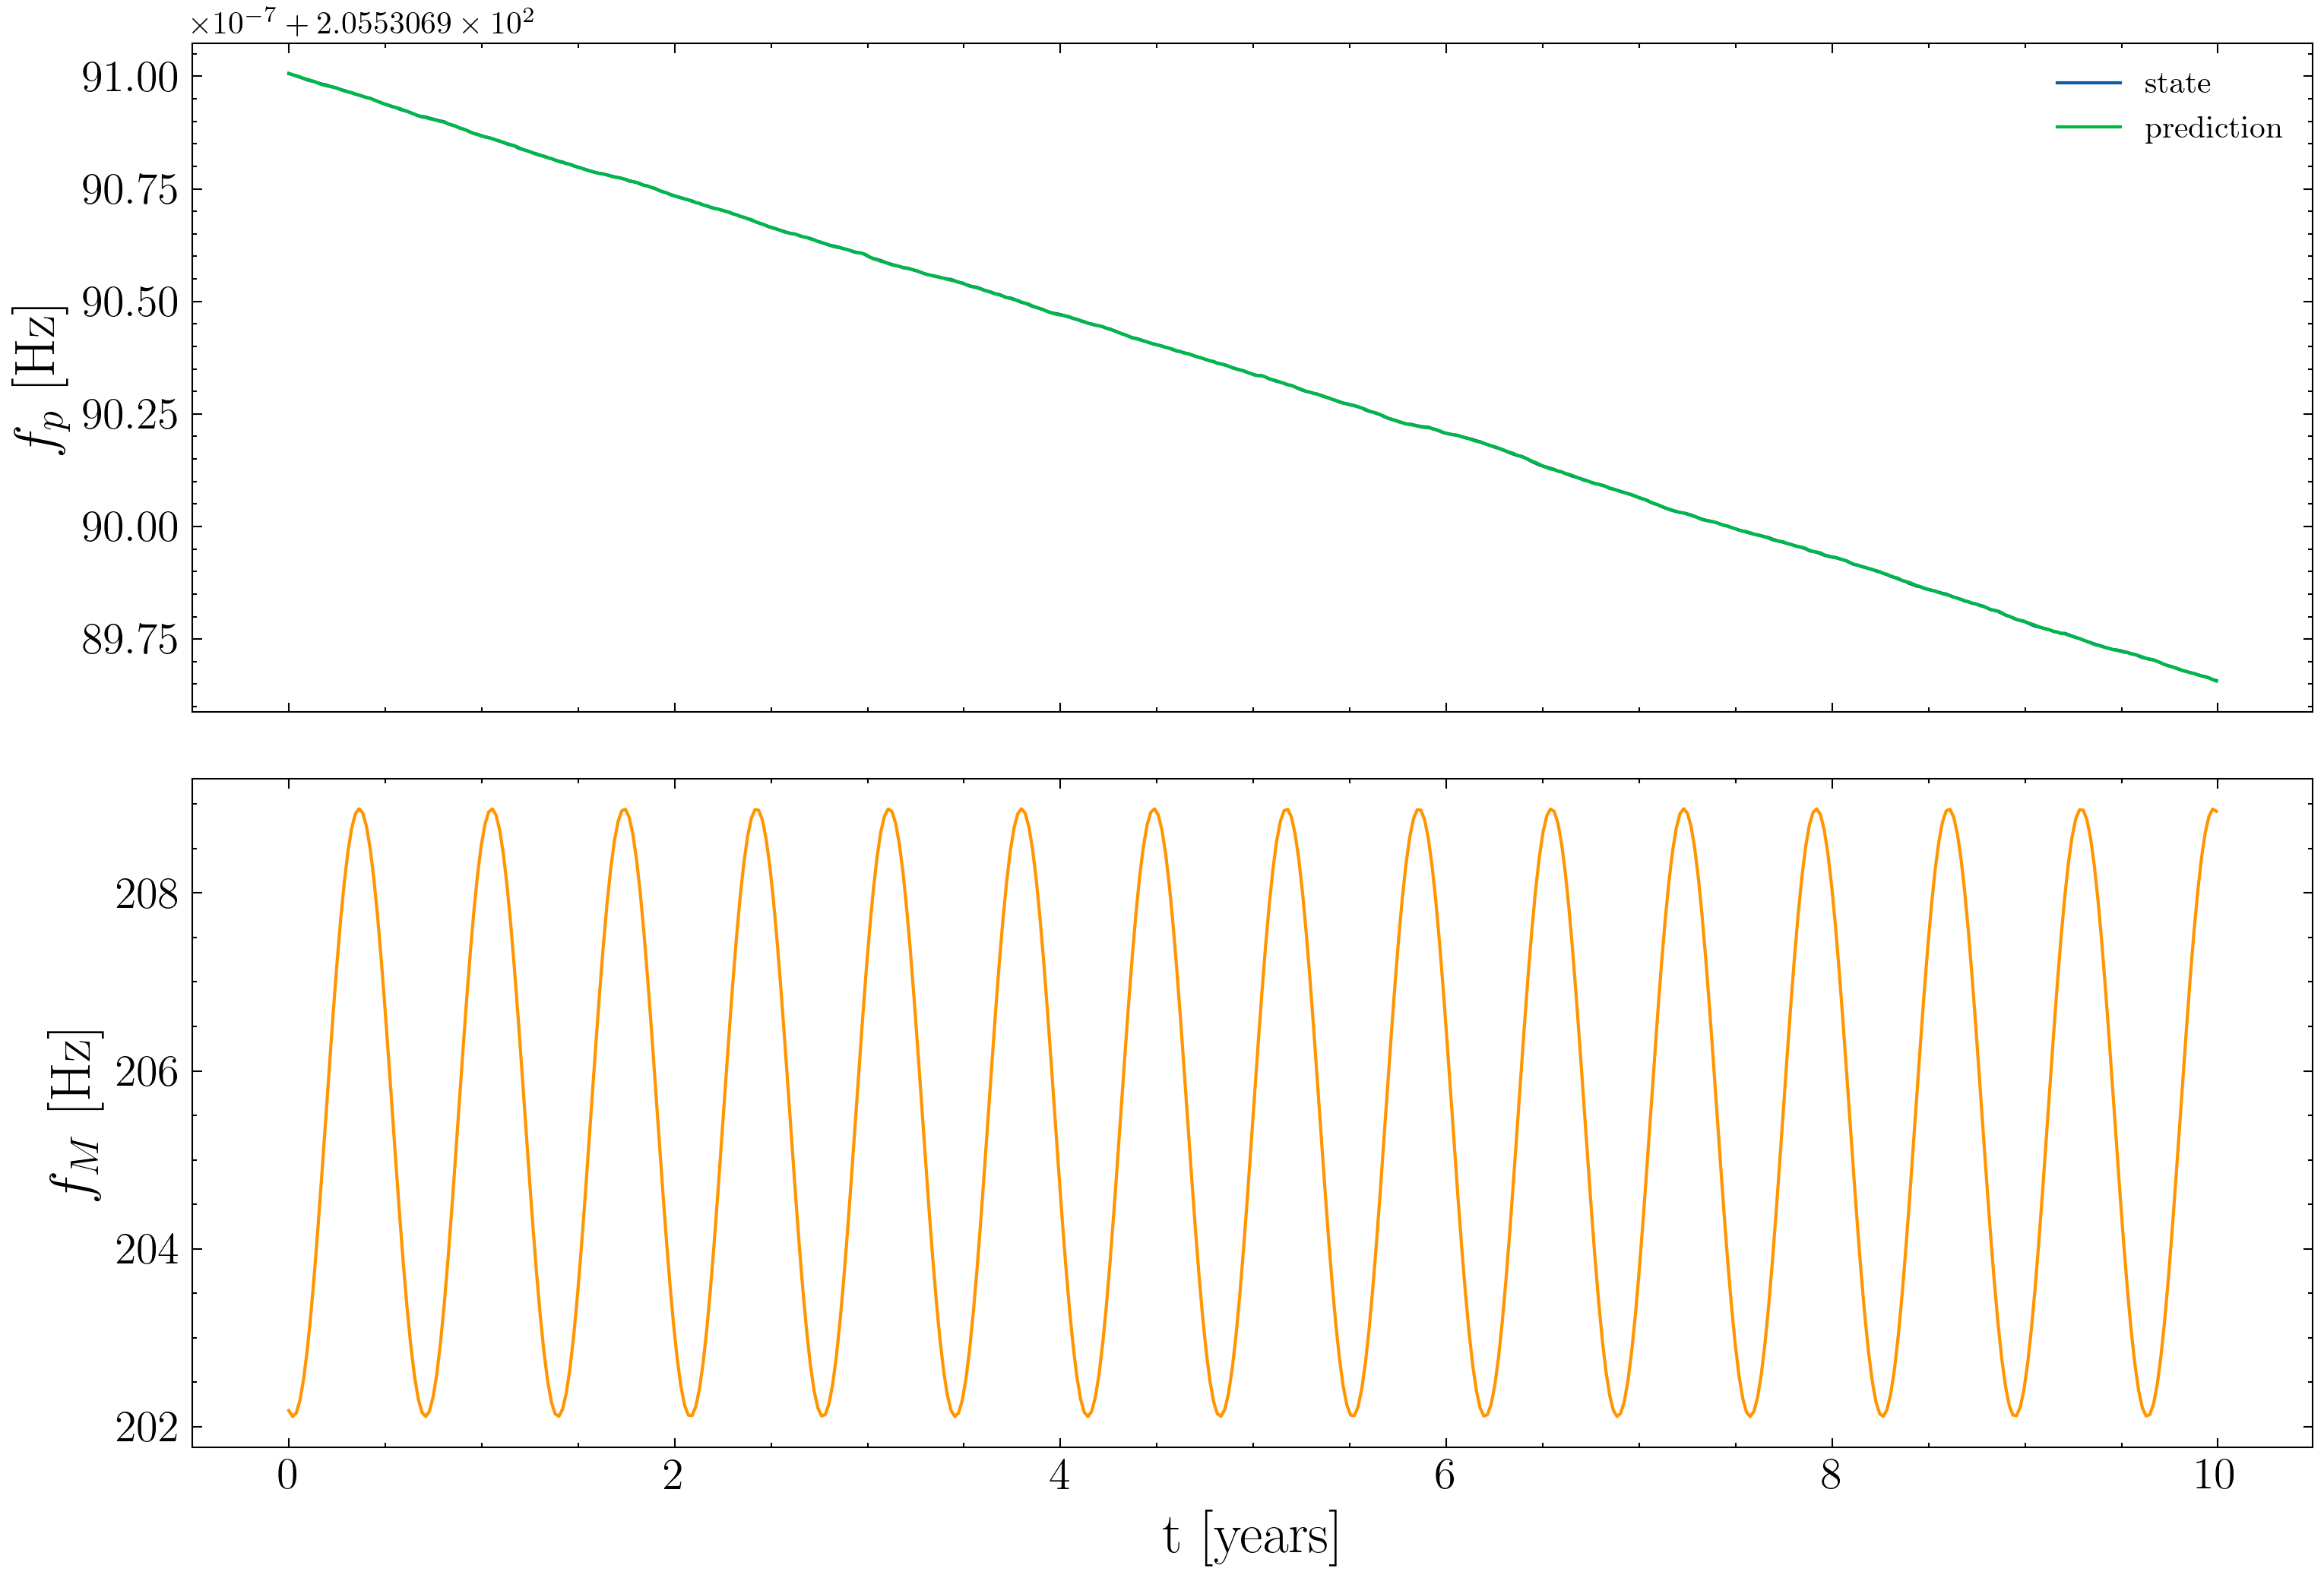
\includegraphics[width=\textwidth]{images/KF1}
		\caption{Using correct parameters}
		\label{fig:6MB_BFS}
	\end{subfigure}
	\hfill
	\begin{subfigure}[b]{1\columnwidth}
		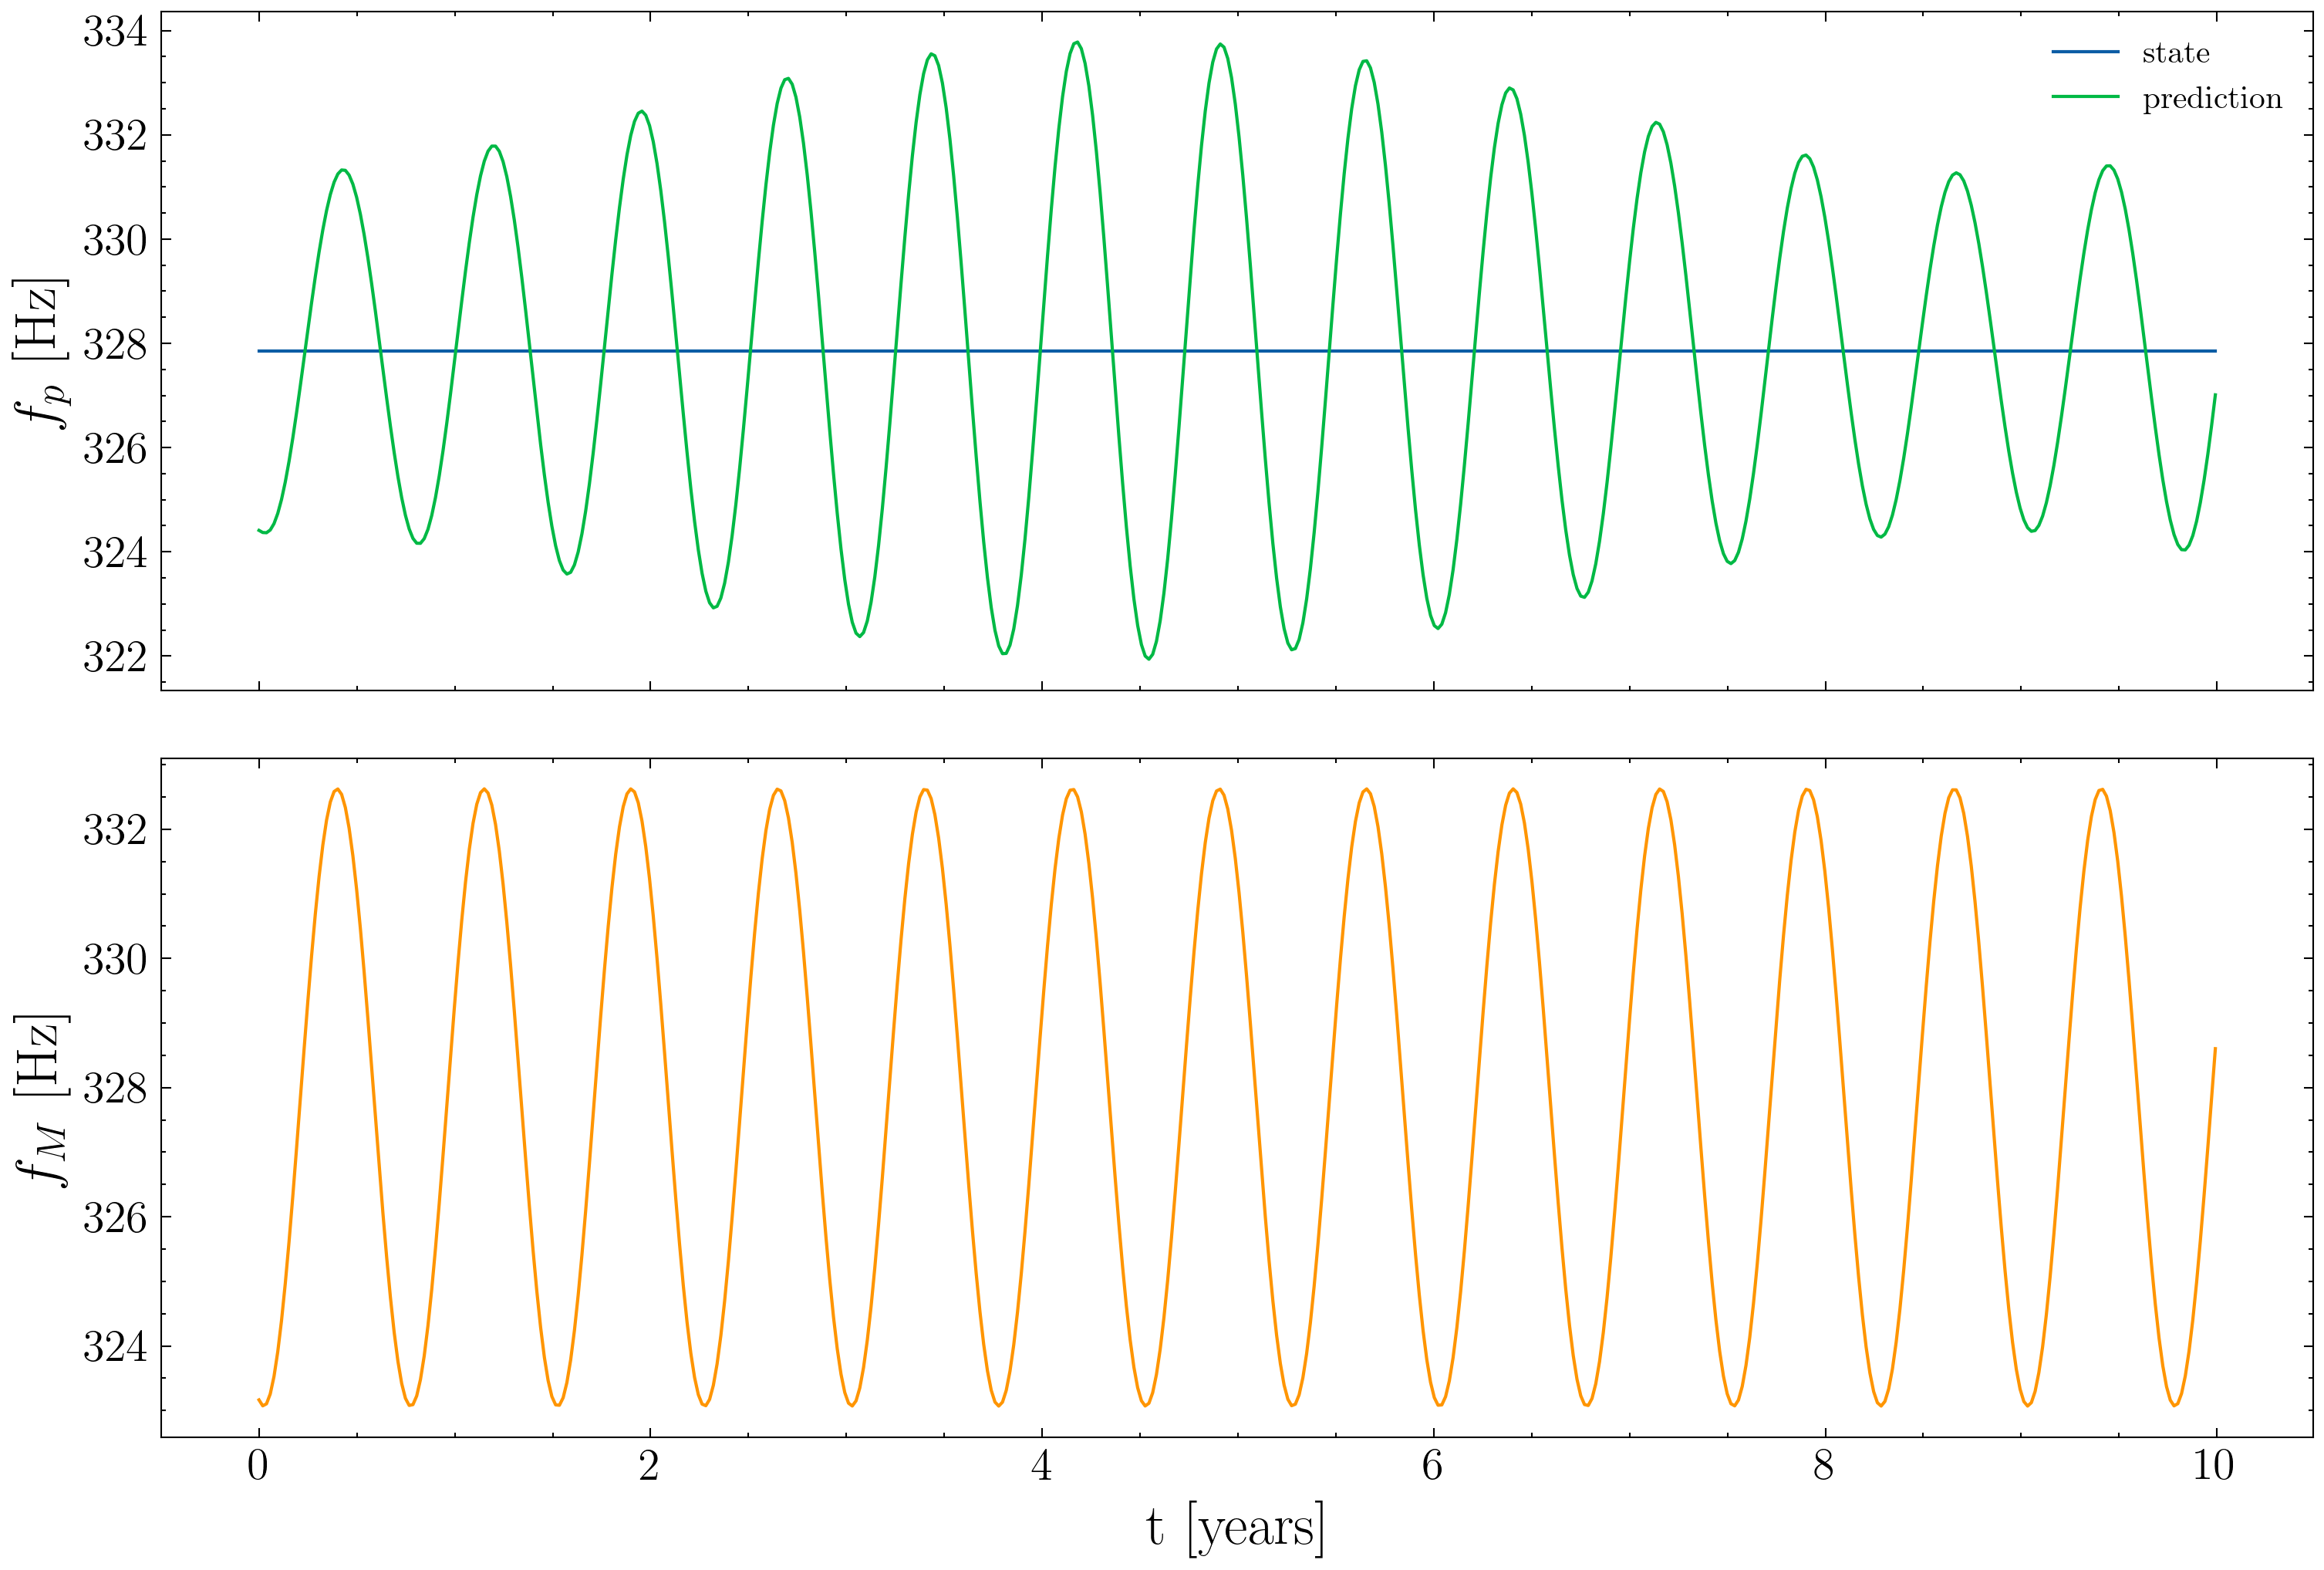
\includegraphics[width=\textwidth]{images/KF2}
		\caption{Using incorrect parameters}
		\label{fig:25MB_bfs}
	\end{subfigure}
	\caption{Application of a Kalman filter to recover the intrinsic frequency states (top panels) given a measured frequency signal (bottom panels) which has been modulated by the presence of a gravitational wave. In the case where the parameters of the filter are accurate (subfigure (a)) the underlying states are also recovered accurately. Conversely, when the parameters fed to the filter are inaccurate (subfigure (b)) the filter cannot recover the state. \textcolor{red}{TK: this needs to be just one stacked figure.}}
	\label{fig:four figures}
\end{figure*}

The Kalman filter \citep{Kalman1} is a algorithmic technique for recovering a set of system state variables, $\bar{x}$, given some noisy measurements, $\bar{z}$. It is a common technique in signal processing that has also been applied more recently with great success in astrophysics \citep[e.g.][]{Meyers2021,Melatos2023}. The linear Kalman filter operates on measurements that are related to states via a linear transformation
\begin{equation}
	\bar{z} = \bar{H} \bar{x} + \bar{v}
\end{equation}
where $\bar{H}$ is the measurement matrix and $\bar{v}$ a Gaussian measurement noise. The underlying states are the solutions to the state-space equation 
\begin{equation}
	\dot{\bar{x}} = \bar{F} \bar{x} + \bar{G}\bar{u} + \bar{w}
\end{equation}
for the system dynamics matrix,$\bar{F}$,  control model $G$, control vector $\bar{u}$, and $w$ a stochastic zero-mean process. By comparison with the preceding equations, Eqs. 	\ref{eq:state1} - 	\ref{eq:state2}, it is immediately obvious how our state space model maps onto the Kalman filter structure. Specifically, our states are just the $N$ intrinsic pulsar frequencies $\bar{x} = (f_1,f_2,...f_N)$ whilst our measurements are the $N$ measured pulse frequencies $\bar{z} = (f^{(M)}_1,f^{(M)}_2,...f^{(M)}_N)$. If we specialize to the case of constant time sampling between our observations, $\Delta t$, then for our formulation the components that make up the Kalman filter are as follows: 
\begin{equation}
	F_i = F_{i+1} = e^{-\gamma \Delta t}
	\label{eq:fmatrix}
\end{equation}
\begin{align}
	T_i &= \int_{t_i}^{t_{i+1}}  e^{A (t_{i+1} - t')} N(t') dt' \\
	    & = f_{\rm EM}(0) + \dot{f}_{\rm EM}(0)  (\Delta t + t_i) - e^{-\gamma \Delta t} (f_{\rm EM}(0) + \dot{f}_{\rm EM}(0)t_i)
\end{align}
\begin{equation}
	H_i = 1 -A(\theta_{\rm GW}) \cos(-\Omega t_i (1 + n\cdot q ) + \Phi_0)
\end{equation}
where the $i$ subscript labels the value at the $i$-th timestep, and $A$ is a constant that is given by  Eq. \ref{eq:state2}. \newline 


\noindent The Kalman filter includes the effect of process noise $\bar{w}$ and the measurement noise $\bar{v}$ via the definition of a process noise matrix $Q = E[w w^T]$ and a measurement noise matrix $R = E[v v^T]$, which have the discrete form,
\begin{equation}
	Q_i  \delta_{ij}= \langle \eta_i \eta_j^T \rangle = \frac{- \sigma^2}{2 \gamma} \left( e^{-2 \gamma \Delta t} -1\right)
\end{equation}
\begin{equation}
	R_i = R_{i+1} = \Sigma^2
	\label{eq:rmatix}
\end{equation}
The above equations, Eqs. \ref{eq:fmatrix} - 	\ref{eq:rmatix}, apply to an operation on a single state. The extension to $N$ states is straightforward, since one just needs to construct a diagonal matrix for each of the Kalman components where each non-zero element corresponds to a separate pulsar frequency. For our formulation we are concerned only with the linear Kalman filter since the measurements are a linear function of the states and the state transitions are also linear. Extension to non-linear problems is straightforward using either an extended Kalman filter \citep{zarchan2000fundamentals}, the unscented Kalman filter \citep{882463van} or the particle filter \citep{Simon10}. For a full review of the  Kalman filter equations in an astrophysical context, which may be unfamiliar to some, we refer the reader to the appendices of \cite{Melatos2023} and  \cite{Meyers2021}. \newline 



\noindent In order for the Kalman filter to function successfully, the parameters of the model, which appear in the various Kalman matrices, must be accurate. Erroneous or inaccurate parameters lead to inaccurate predictions of the underlying states (e.g. Fig \ref{fig:four figures}). The filter tracks the error in its predictions of the underlying states by projecting the state predictions back into measurement space, $\hat{x} \rightarrow \hat{z}$. These measurement predictions can then be compared against the true observed measurements i.e. $ \epsilon = \bar{z} - \hat{z}$. The Gaussian log-likelihood at timestep $i$, as a function of the parameters is,
\begin{eqnarray}
	\log \mathcal{L}_i =  -\frac{1}{2} (N \log 2 \pi + \log \det |S_i| + \epsilon_i^T S_i^{-1} \epsilon_i)
\end{eqnarray}
where $S_i$ is the covariance matrix of the error $\epsilon_i$. The net log-likelihood is simply the sum over all timesteps. 


\subsection{Nested Sampling}\label{sec:nested_sampling}
Nested Sampling \citep{Skilling} is an integration algorithm used for evaluating integrals of the Bayesian evidence form,
\begin{eqnarray}
	Z = \int \mathcal{L} \pi (\theta) d \theta
\end{eqnarray}
where $\pi (\theta)$ is the prior which is a function of a set of unknown parameters $\theta$. The primary advantage of nested sampling is the ability to compute this evidence integral, which is key for model selection, and proves difficult without considerable extra cost for the usual Markov Chain Monte Carlo (MCMC) approaches. Nested sampling is also typically less computationally intensive than MCMC and can handle multi-modal problems \citep{Ashton2022}. For these reasons, it has enjoyed widespread adoption in the physical sciences, particularly within the cosmological community \citep{Mukherjee2006,Feroz2008,Handley2015}, but has also commonly been applied in astrophysics \citep{UltraNest2021}, particle physics \citep{proceedings2019033014} and materials science \citep{2009arXiv0906materials}. Within this work we also use nested sampling for parameter estimation and model selection. \newline 


\noindent Multiple nested sampling libraries exist. For gravitational astrophysics it is common to use the dynesty sampler CITE, via the Bilby gravitational wave inference library and we continue to follow this precedent. 
\textcolor{red}{TK: we may end up not even using Bilby/dynesty so leaving this section unfilled for now. Do we need a very short description of how nested sampling works?}



\subsection{PTA pulsars}\label{sec:pta_pulsars}
\begin{figure}
	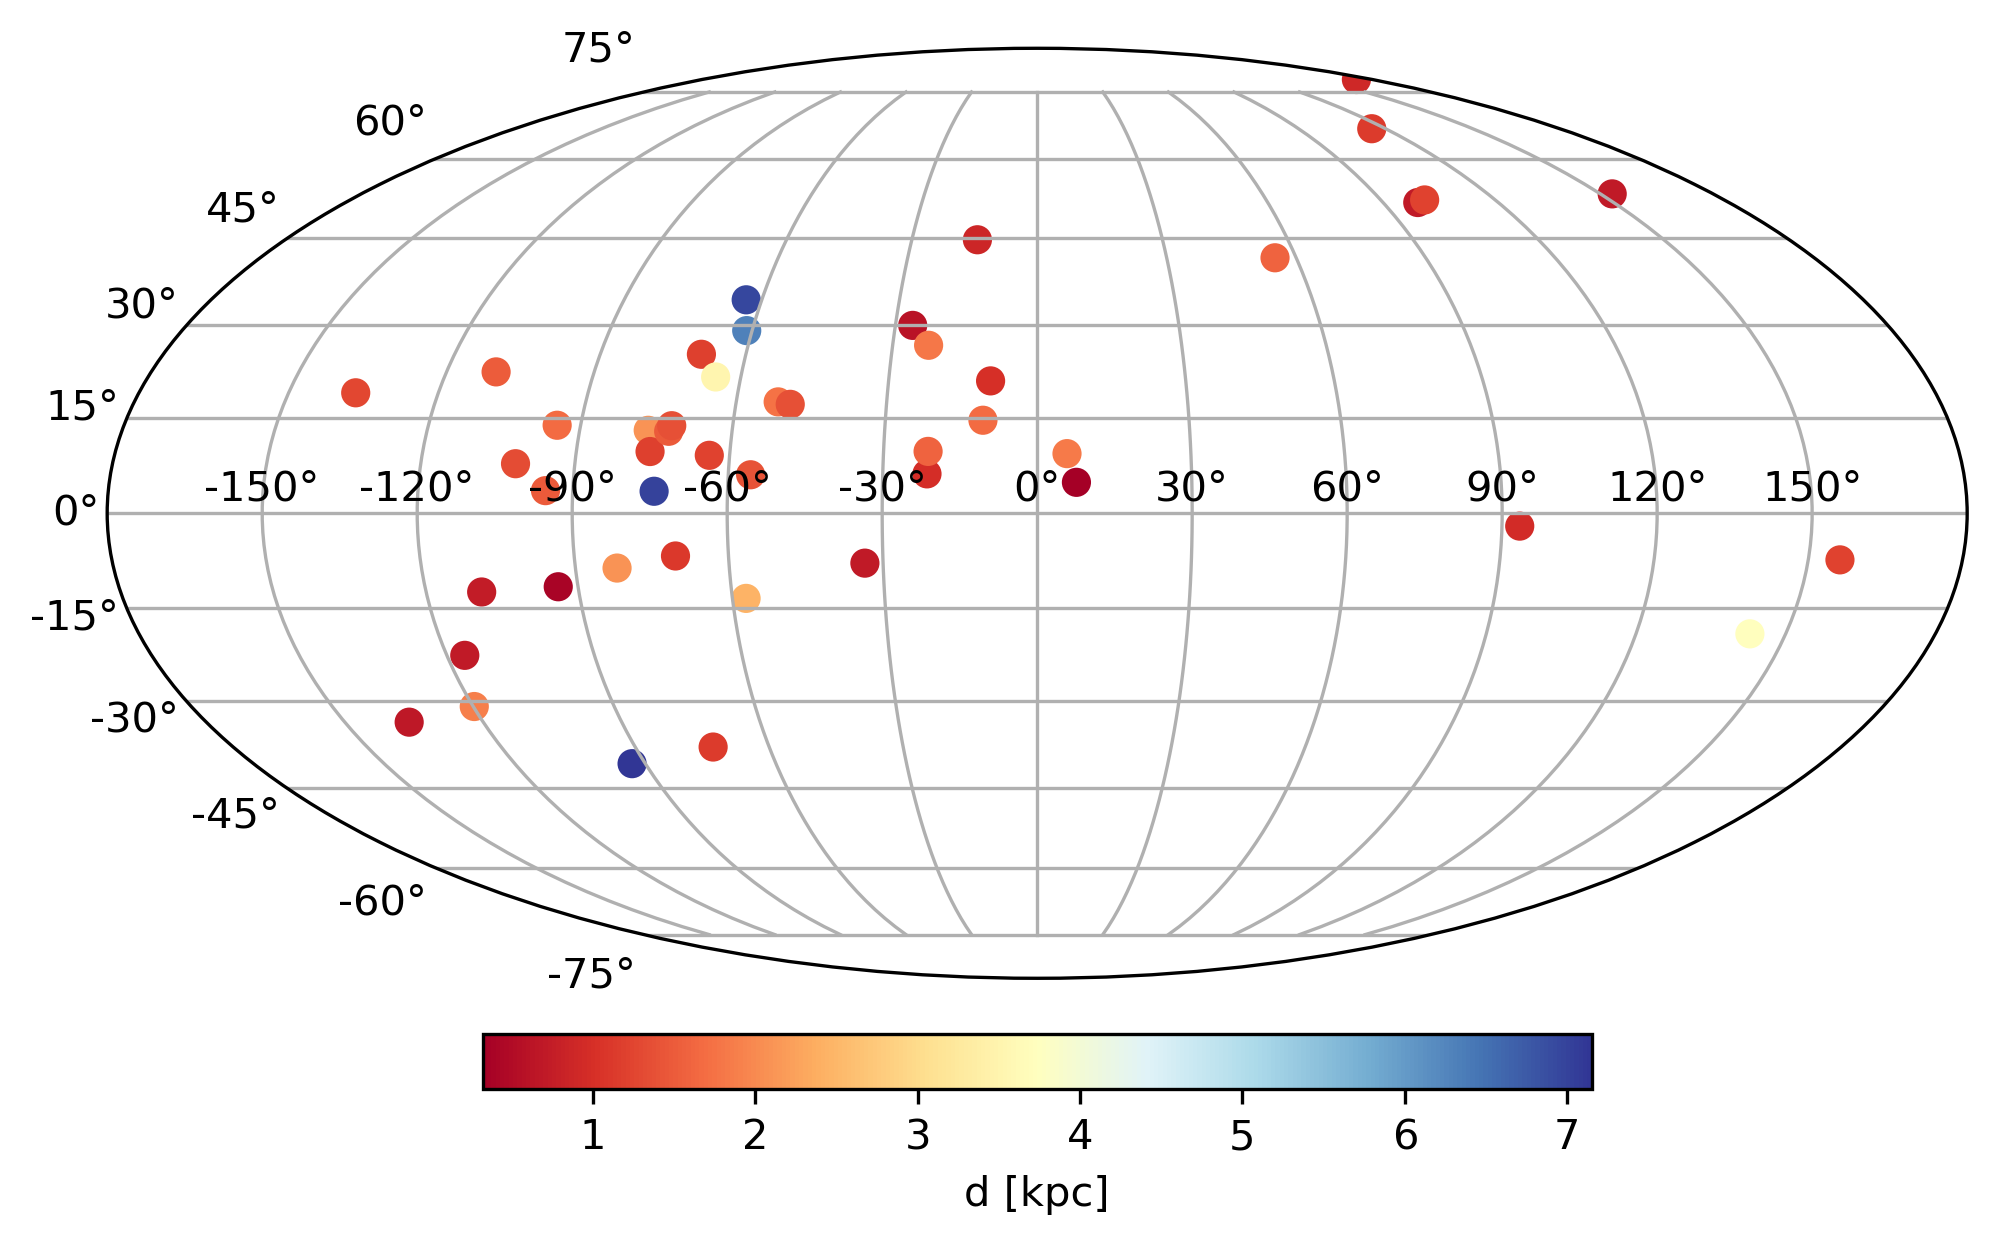
\includegraphics[width=0.8\columnwidth]{images/pulsars}
	\caption{Spatial distribution and distances of NANOGrav pulsars}
	\label{fig:pulsar_distrib}
\end{figure}
\noindent With our Kalman filter and nested sampling techniques in hand, in order to proceed it is necessary to specify a PTA configuration. As discussed, multiple separate PTA detectors exist under the umbrella of the IPTA. Going forward we will take the 47 pulsars that make up the NANOGrav PTA \citep{2020ApJ...905L..34A}. NANOGrav is selected simply as a well-representative example of the typical pulsars that make up a PTA. Our results and formulation are not contingent on the choice of PTA, and naturally extend to other PTAs or PTAs with more pulsars.  \newline 



\noindent Within our state-space formulation, the pulsar evolution is governed by a set of 5 parameters, $\bar{\theta}_{\rm PSR}$ for each pulsar. The parameters $f_{\rm EM} (0) $,$ \dot{f}_{\rm EM} (0)$ and $d$ are well specified via existing pulsar datasets. We take the frequency and frequency derivative as returned from the pulsar datasets to simply be the values now at $t=0$. The pulsar distances are also known, though less well constrained. Going forward we take the distances retuned from the datasets as the true values of the pulsars that make up our synthetic PTA. The specification of $\gamma$ and $\sigma$ are more involved. $\gamma$ specifies an effective timescale of reversion to the mean \textcolor{red}{TK: Need some discussion and though on how to choose these two parameters to be astrophysically reasonable c.f. A. Vargas}



\subsection{Parameter estimation on synthetic data}\label{sec:param_estimation}
We are now in a position to try to infer the parameters of a GW system. We take our NANOGrav PTA and create a synthetic noisy dataset using the parameters described in Table \ref{tab:toy_example_parameters}.
\begin{table}
	\centering
	\begin{tabular}{lc}
		Parameter & Value  \\
		\hline
		$\omega$       & $5 \times 10^{-7}$  \\
		$\alpha$          & $1.0$  \\
		$\delta$              & $1.0$   \\
		$\psi$              & $2.50$  \\
		$\iota$             & $1.0$  \\
		$\Phi_0$          & $0.20$  \\
		$h$ & 1e-2 \\
		$\sigma_{\rm p}$ & $10^{-13}$ \\
		$\sigma_{\rm m}$ & $10^{-10}$ \\
		$T_{obs}$ & 10 \text{ years} \\
		$\Delta t$ & 7 \text{ days} \\
		\hline
	\end{tabular}
	\caption{GW parameters used for generating synthetic data. There is nothing special about these parameters - they are just chosen arbitrarily.}
	\label{tab:toy_example_parameters}
\end{table}
\noindent Given this synthetic data, we can try to use our KF + NS approach to recover some of the parameters. The results for inference on 5 parameters, $\omega. \Phi_0, \psi, \iota, h$ are shown in Fig \ref{fig:corner}. \textcolor{red}{TK: likelihood plots for each parameter could also be of interest to include here? Need to expand this section greatly for more astrophysical systems and more unknown parameters}
\begin{figure*}
	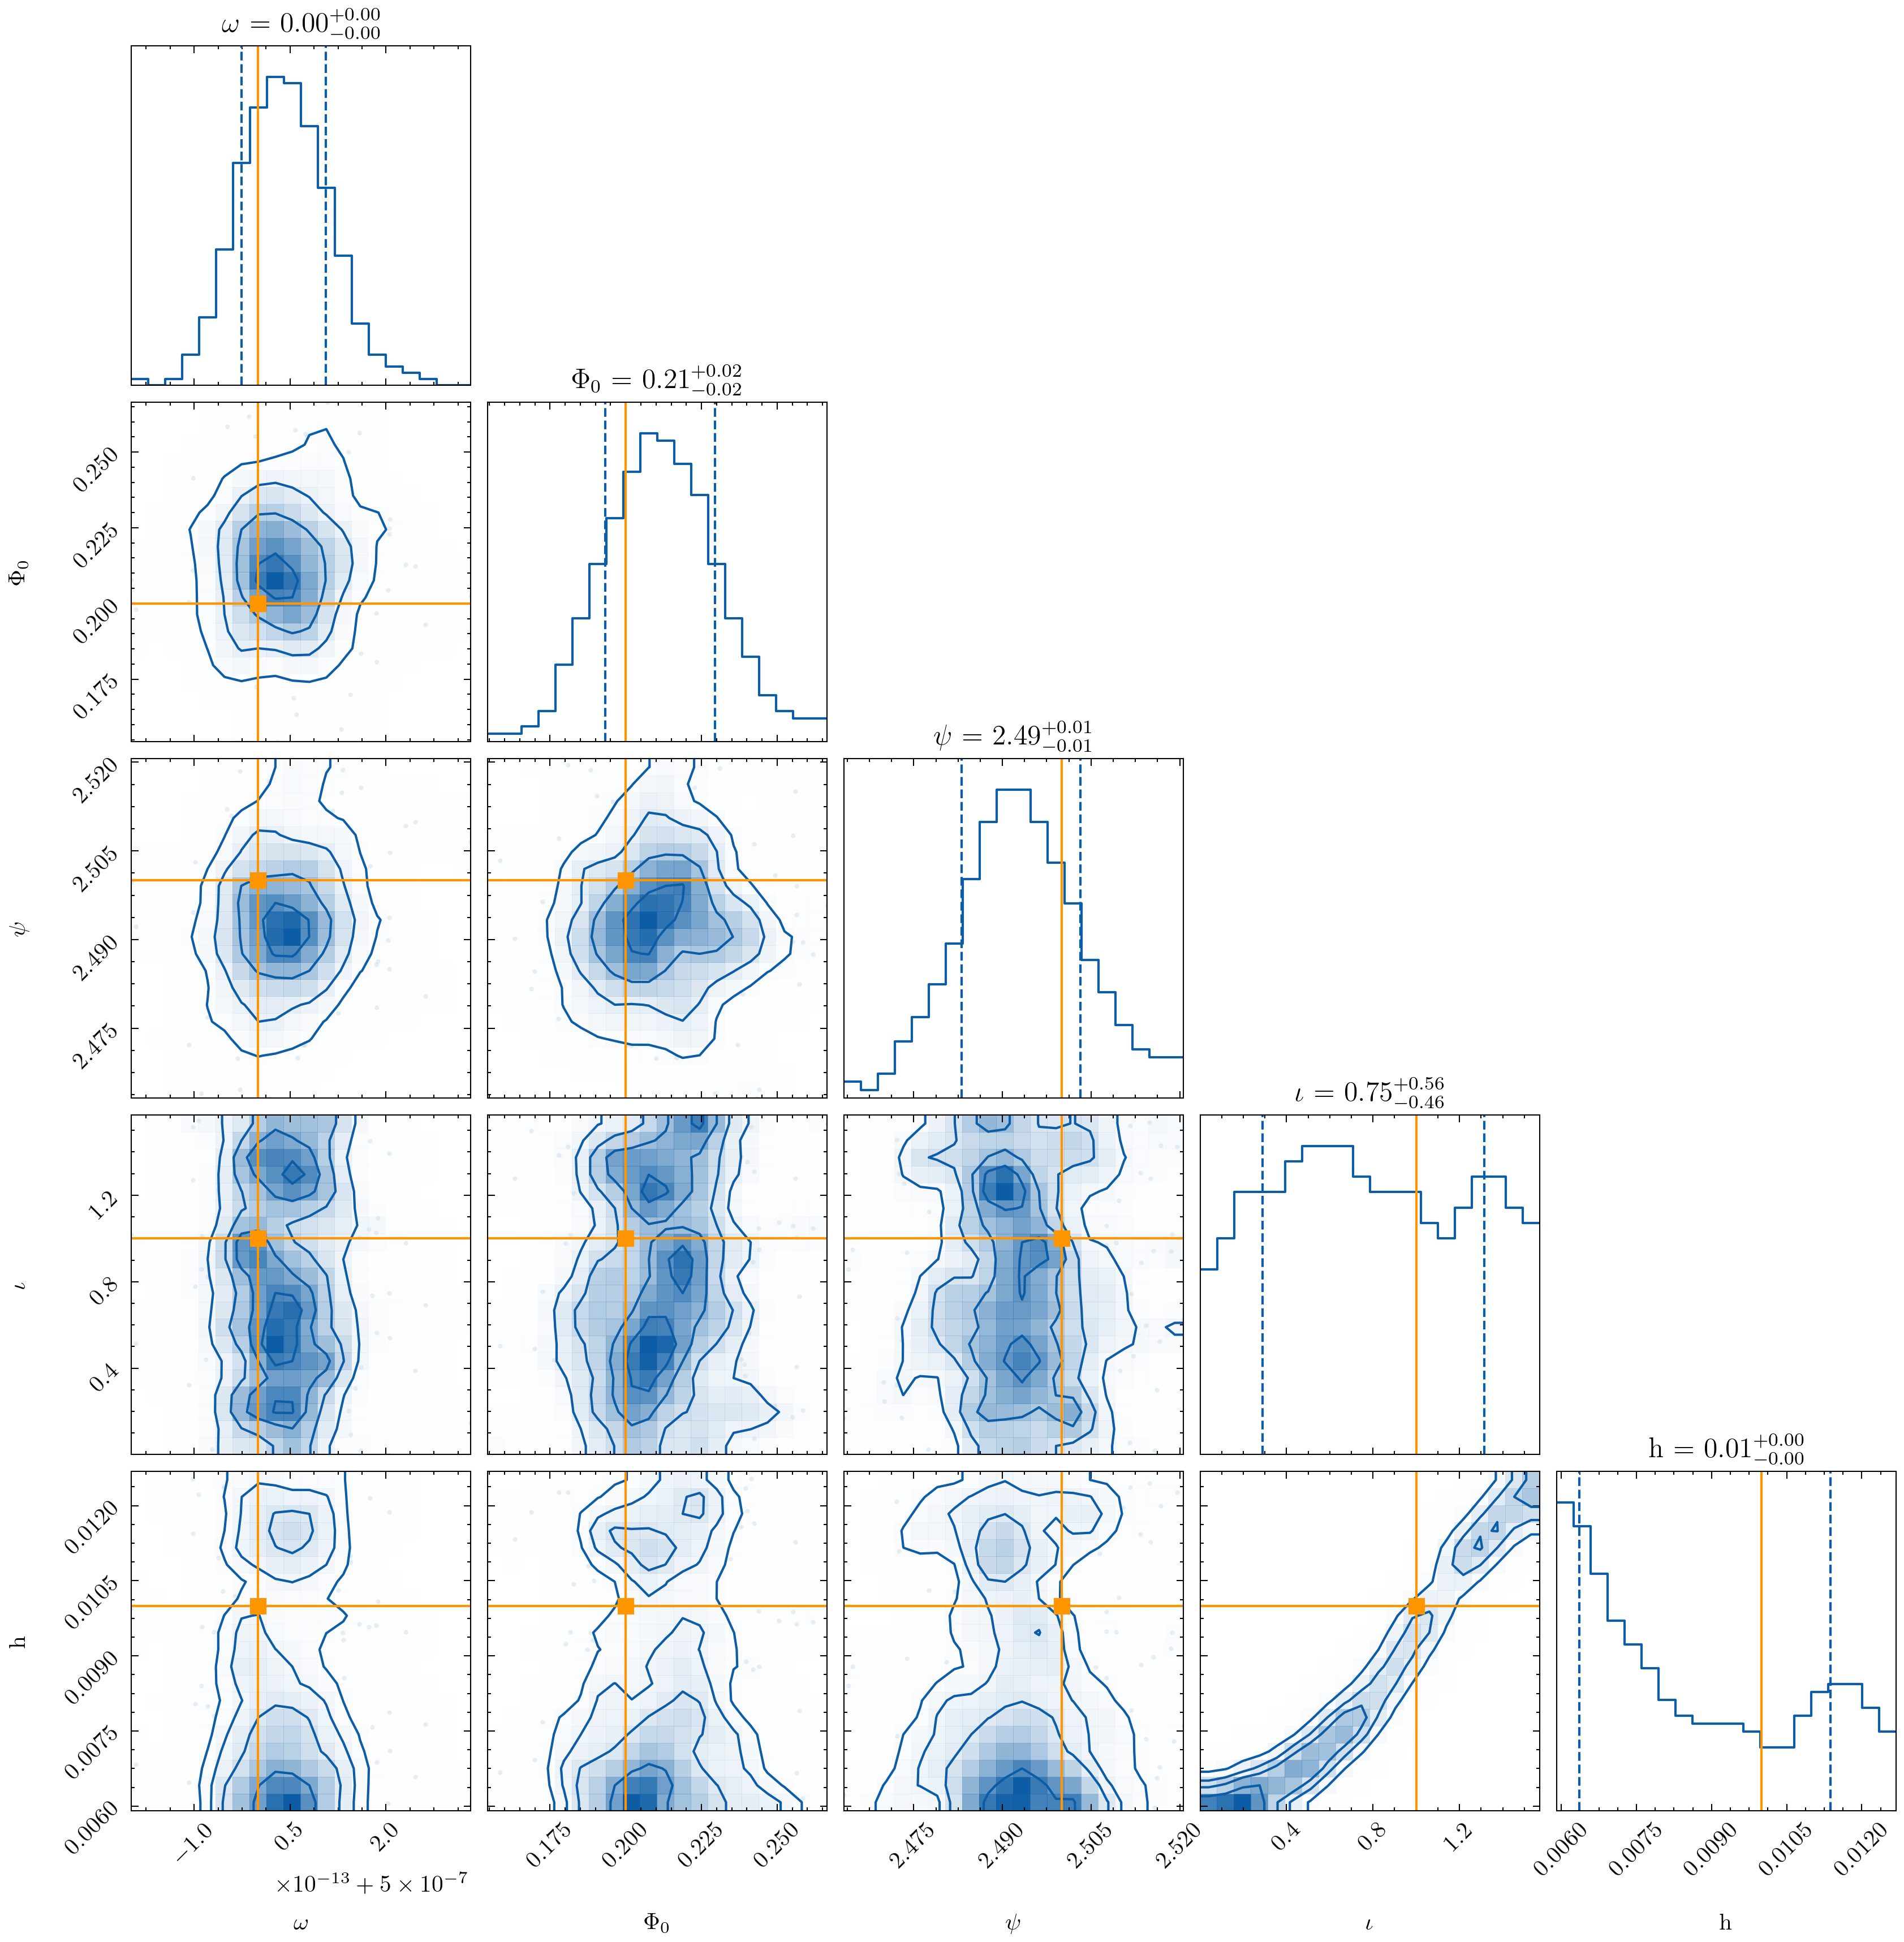
\includegraphics[width=0.8\textwidth]{images/corner_example}
	\caption{Example corner plot. Aside: for this run the $\sigma_p$ value fed to the filter is different from that used to generate the data.}
	\label{fig:corner}
\end{figure*}



\subsection{Detection on synthetic data}\label{sec:detection}

In addition to estimating the parameters of the system, we are also interested in how detectable a GW is using PTA + state space method. We can use our state-space tools  to try to solve the problem of GW detection with a PTA i.e. \textit{"Is there evidence of a GW in my data?"}We can frame this as a model selection procedure where we have two models/hypotheses:

\begin{itemize}
\item Null Model, $M_0$. There is no GW in the data. In this case the measurement model of the Kalman filter simply returns the frequency states i.e. $g(t,\theta)= 0$
\item Alternative model, $M_1$. There is a GW in the data. The measurement model uses the full expression for $g(t,\theta)$
\end{itemize}



In order to accept the alternative hypothesis $M_1$ over $M_0$ there are two approaches we could take:

\begin{enumerate}
	\item The first is a fully Bayesian search over all the parameters for each model, calculating the evidence for each model and then determining the Bayes ratio. This is perhaps the most consistent way, but it is obviously expensive and at this stage we are keen to explore how detectability varies with e.g. GW strain.
	\item The second method is to recognize that $M_0$ and $M_1$ are hierarchically nested models and we can perform a likelihood ratio test. That is, given the maximum likelihood estimators $\hat{\theta}$ of the true parameters $\theta$, the likelihood of each model can be calculate. These likelihoods are just  point estimates of the Bayes factor numerator/denominators. They can then be compared via the likelihood ratio $\Lambda$. 
\end{enumerate}
Given the cheap cost we proceed with the second method. For the likelihood ratio test we do not perform any kind of maximum likelihood search over the parameters for each of the models. Instead we just artificially set the maximum likelihood estimators to be equal to the true parameters of the system i.e. $\hat{\theta} = \theta$. We assume that any maximum likelihood algorithm would converge to these parameters. This is obviously an oversimplification but will serve our purposes for now. \newline 


\noindent Interpreting the likelihood ratio $\Lambda$ also needs some consideration, since we have to account for the increased model complexity of $M_1$. Bayes factors penalise complexity by construction since one must integrate over a larger parameter space. There are many different ways to do this, AIC, BIC, Wilks Theorem... \newline 



\noindent 





\begin{figure}
	%\centering % Not needed
	\begin{subfigure}[b]{1\columnwidth}
		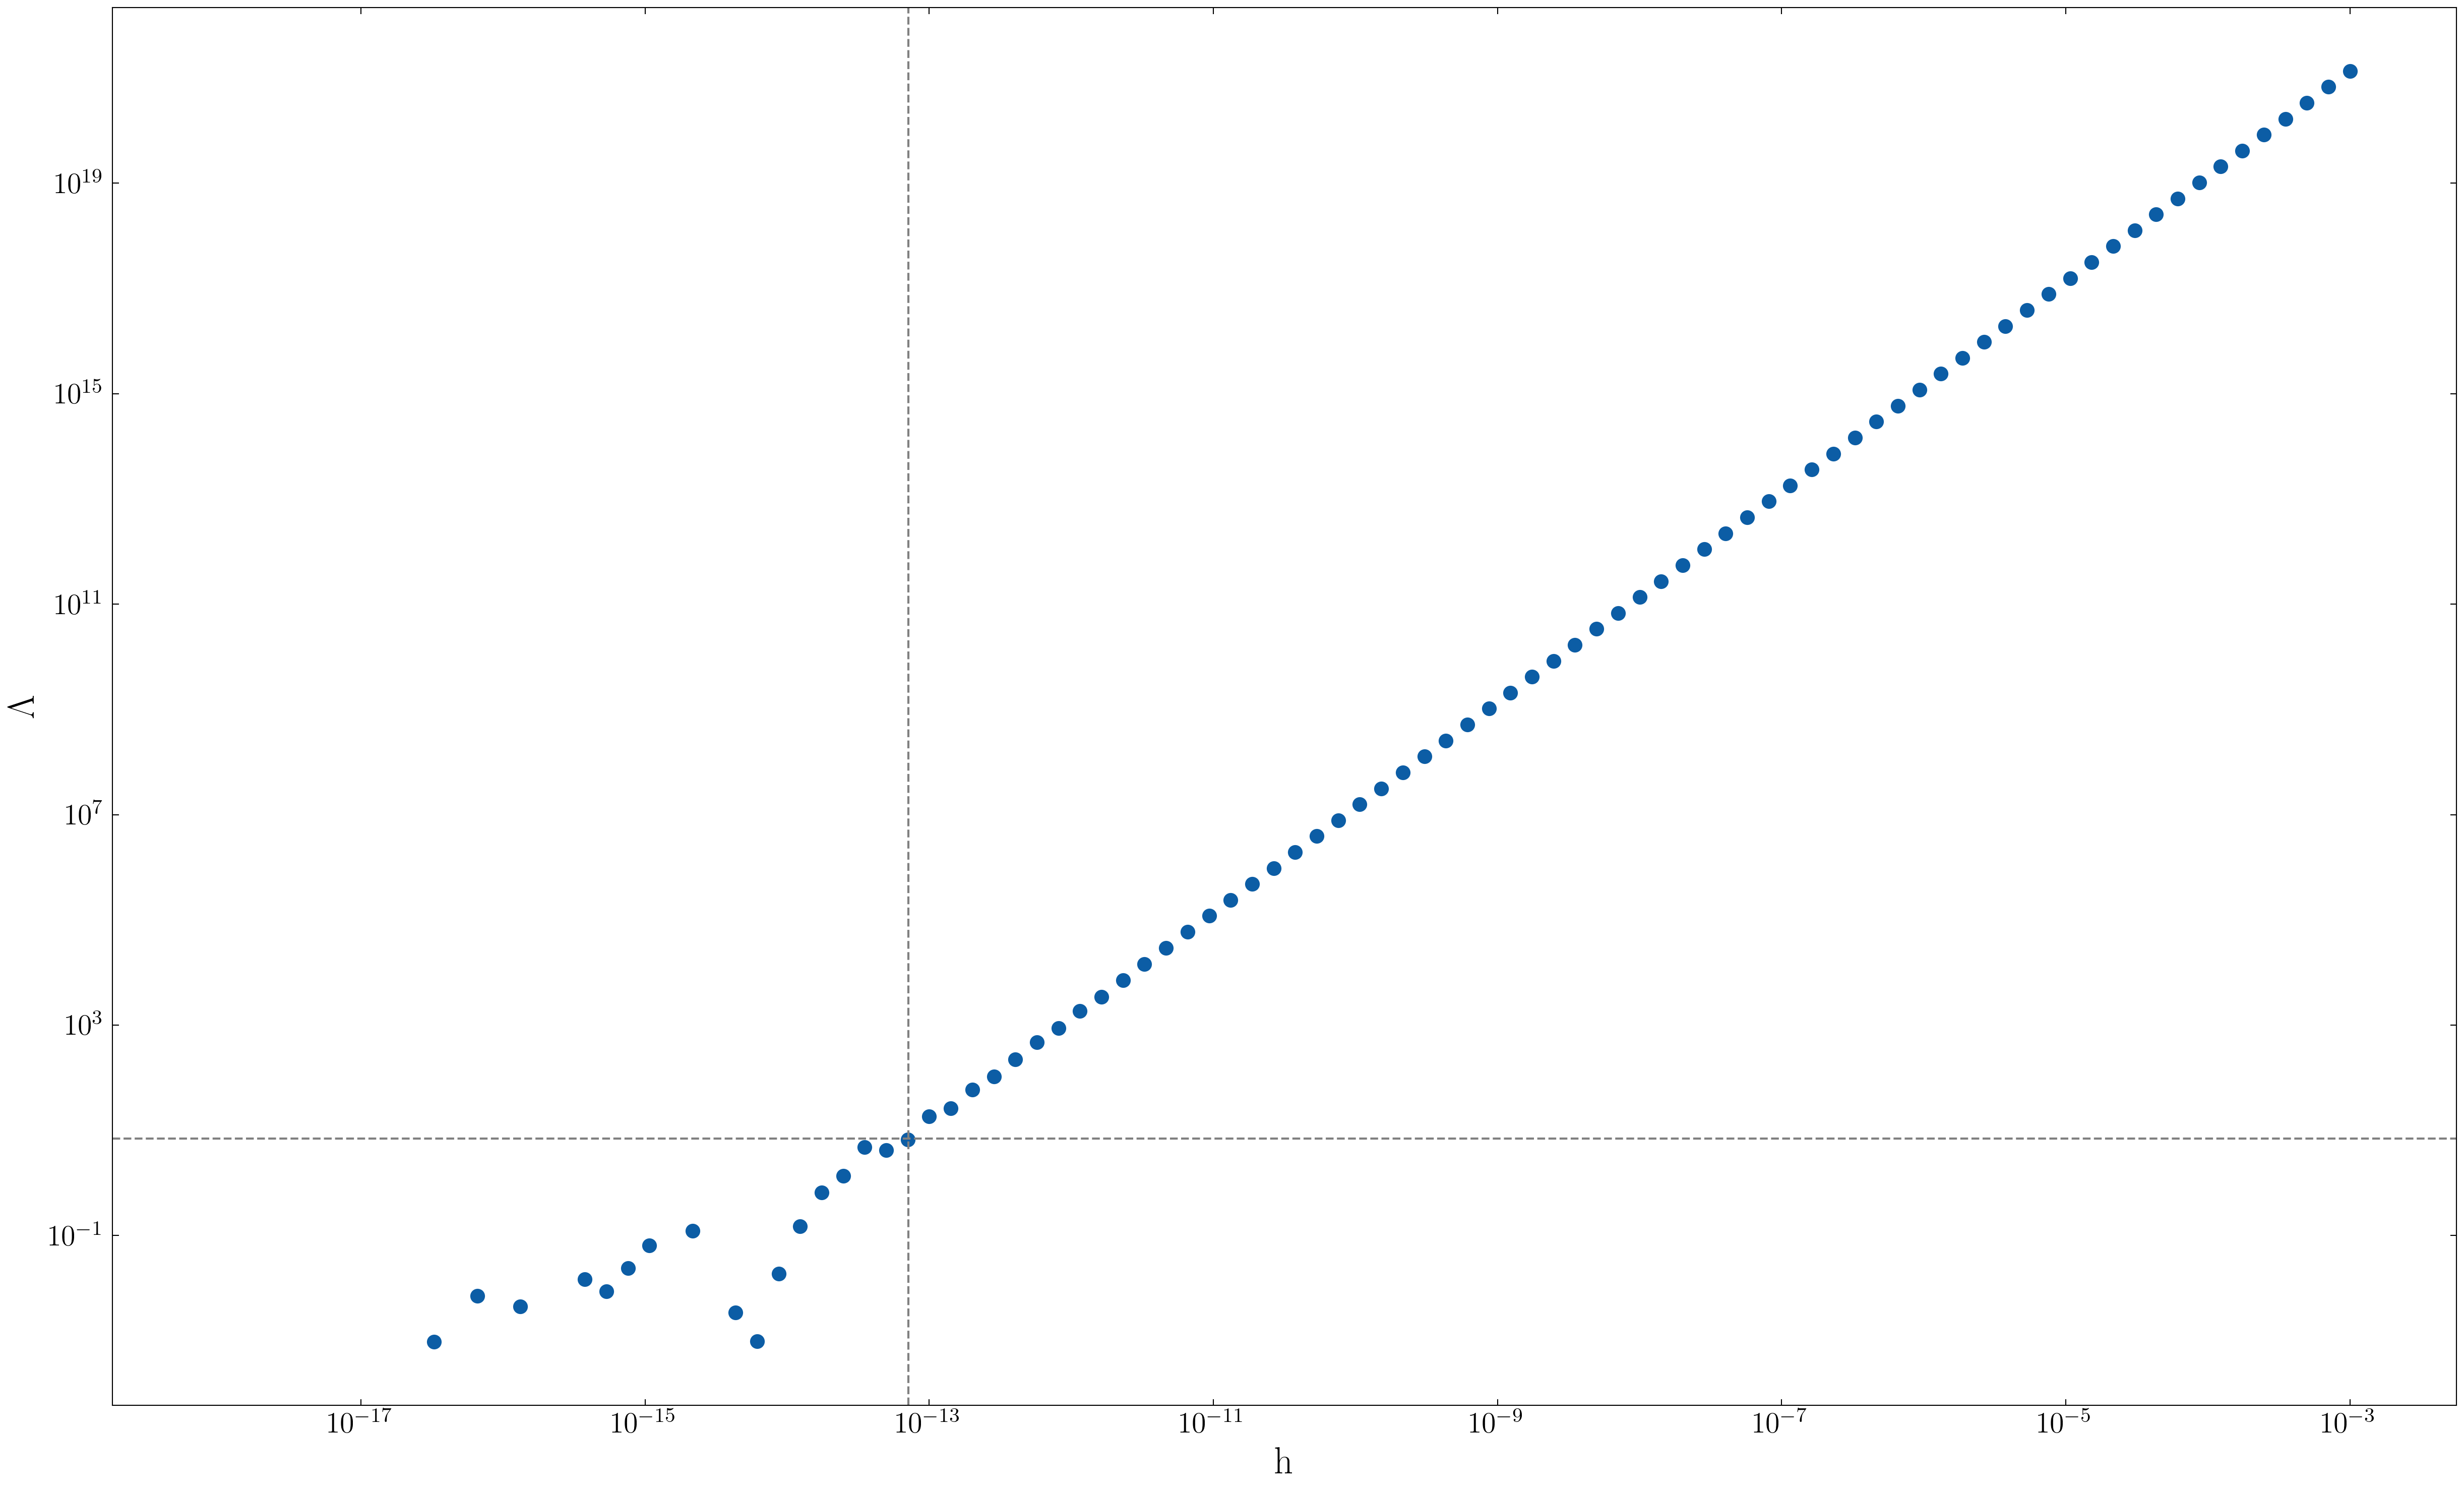
\includegraphics[width=\textwidth]{images/snr_canonical}
		\caption{}
		\label{fig:6MB_BFS}
	\end{subfigure}
	\\
	\begin{subfigure}[b]{1\columnwidth}
		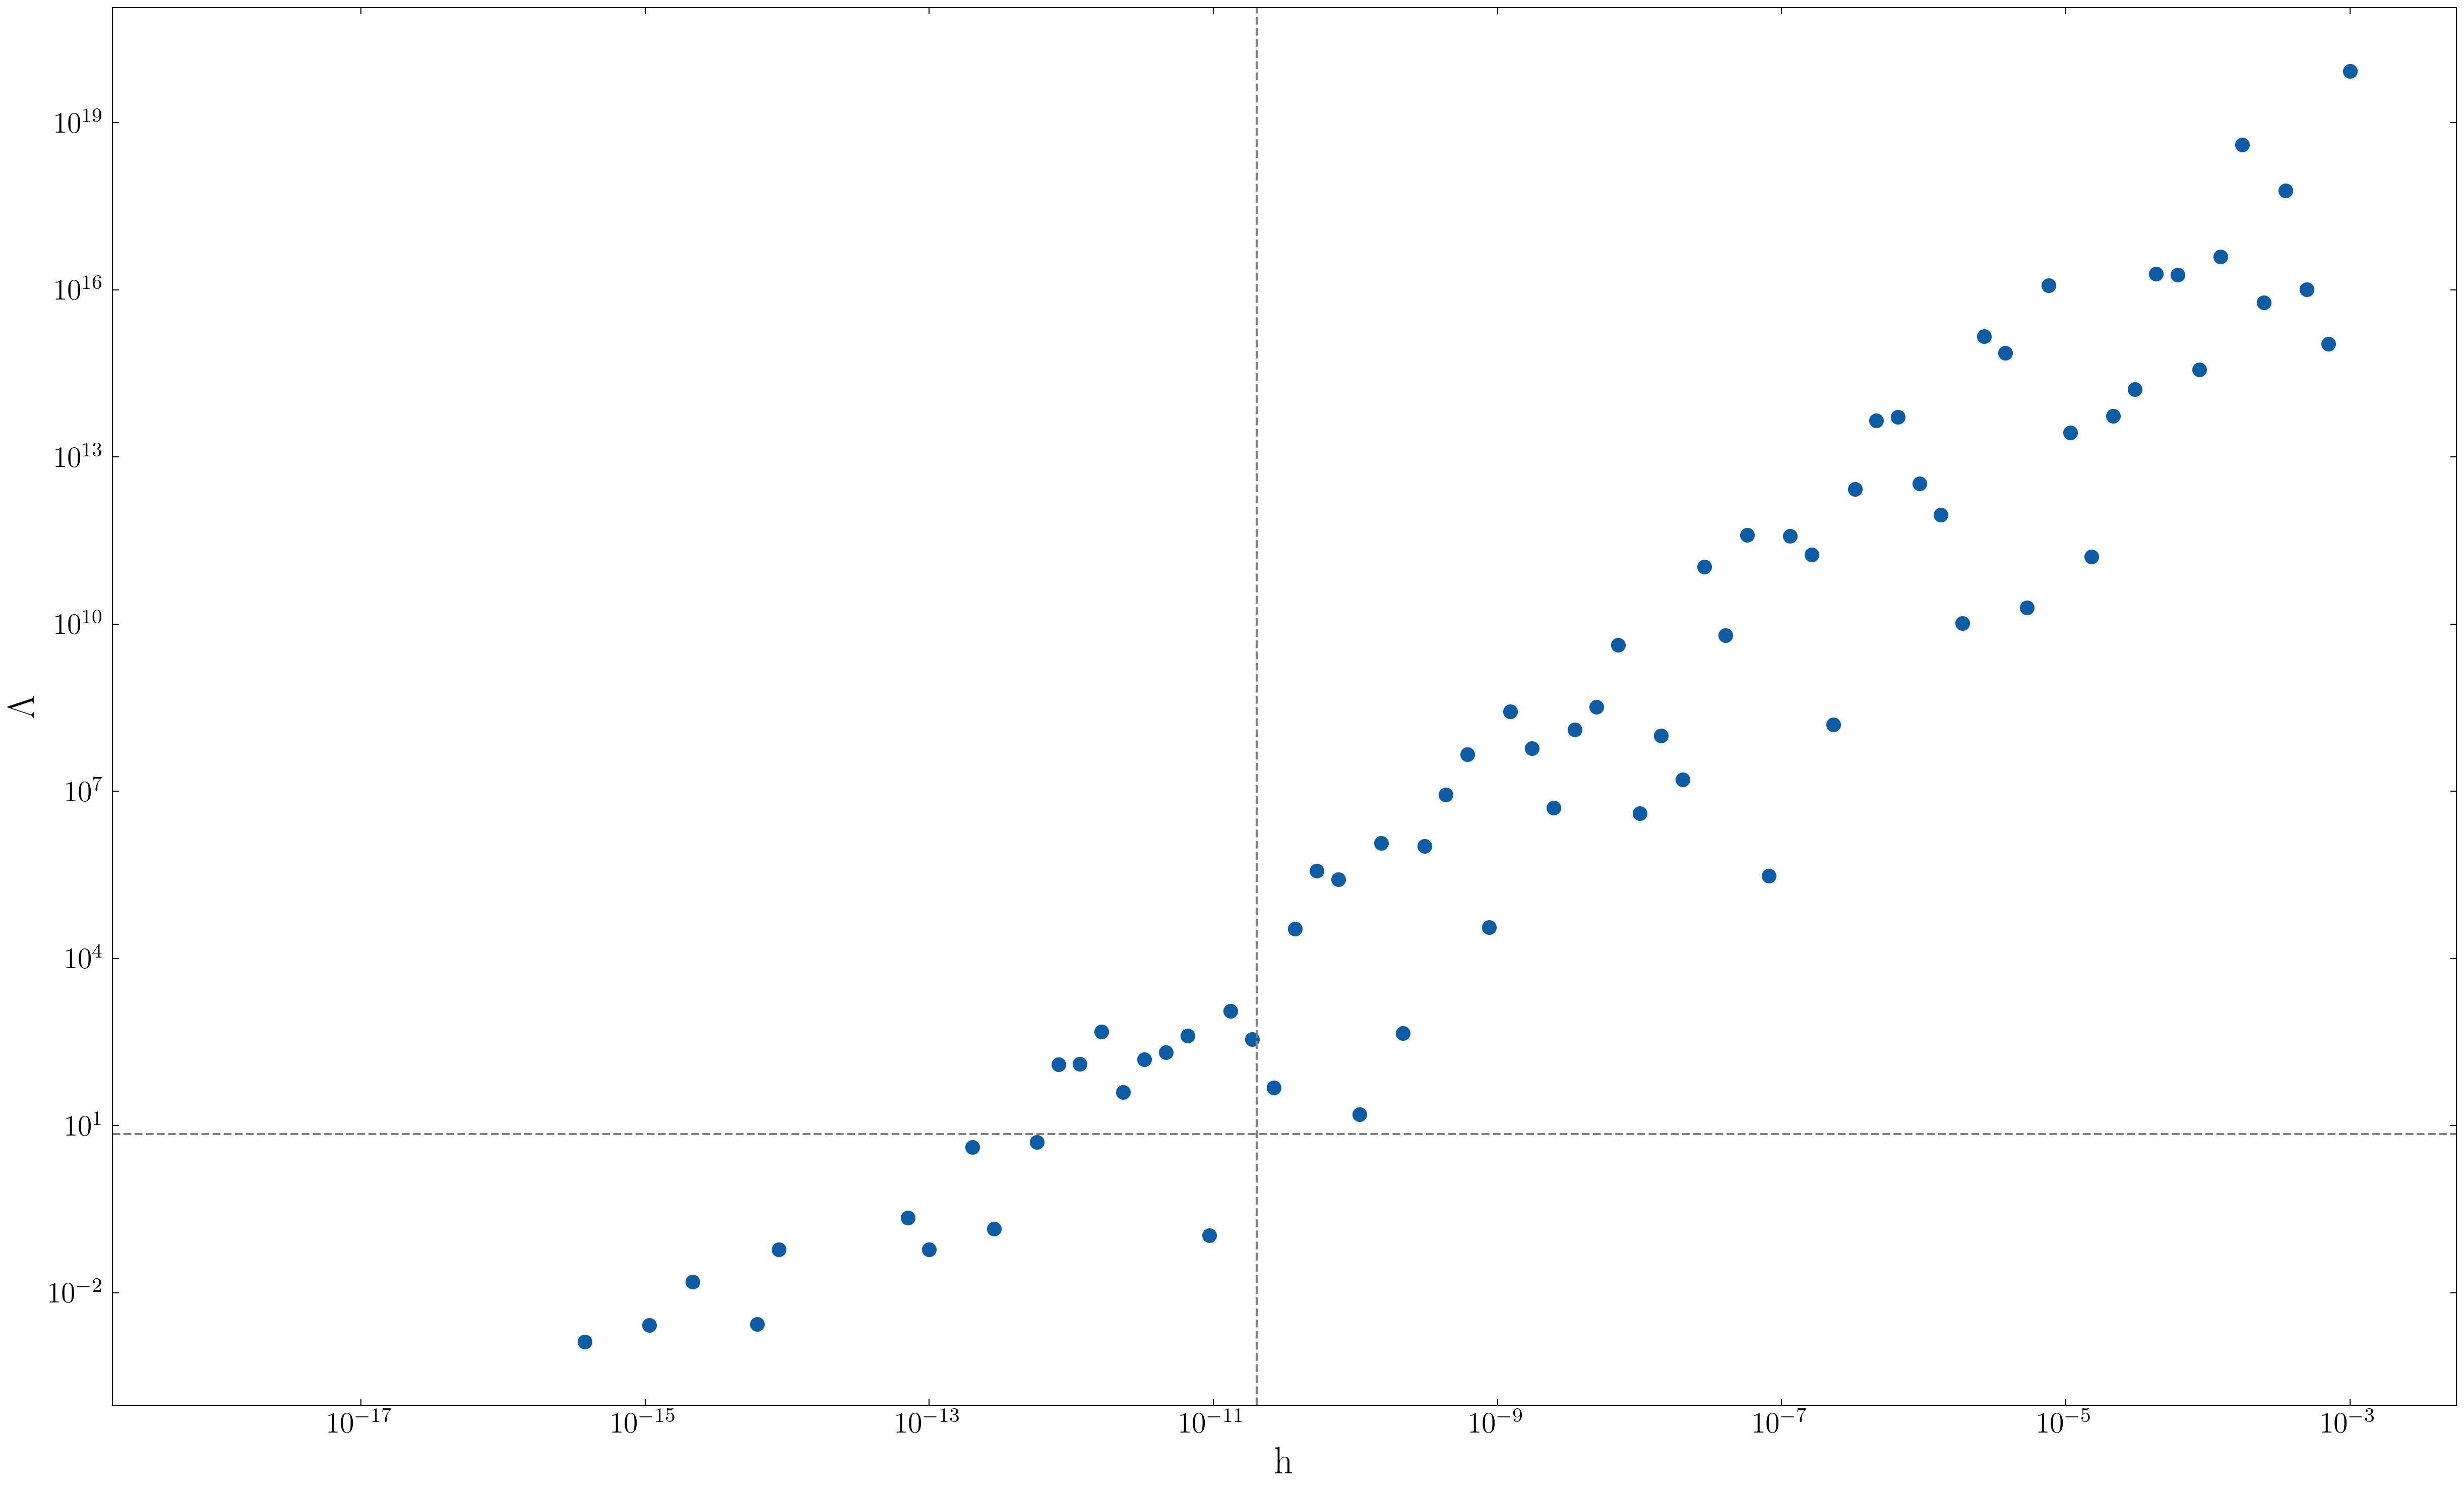
\includegraphics[width=\textwidth]{images/snr_canonical_1psr}
		\caption{}
		\label{fig:25MB_bfs}
	\end{subfigure}
	\caption{Likelihood ratio vs strain for \textit{(a)} full PTA and \textit{(b)} a single randomly chosen pulsar. Horizontal dashed line shows the minimum detectable cutoff, vertical dashed line is the corresponding GW strain.}
	\label{fig:snr_detection}
\end{figure}








\section{Discussion}

Points to discuss:

\begin{itemize}
	\item Non constant time sampling? Different pulsars sampled at different times...
\end{itemize}

\section{Conclusion}

Questions 

\begin{itemize}
	\item PTAs like MSPs for small timing noise. Can we get away with large timing noise, and use more pulsars? Some pulsars are more useful than others, e.g. arXiv 2211.03201
	\item Can we also estimate radiometer noise? Is this useful?
\end{itemize}




\subsection{References}
\label{sec:ref_list}





\bibliographystyle{mnras}
\bibliography{example} % if your bibtex file is called example.bib





%%%%%%%%%%%%%%%%%%%%%%%%%%%%%%%%%%%%%%%%%%%%%%%%%%


% Don't change these lines
\bsp	% typesetting comment
\label{lastpage}
\end{document}

% End of mnras_guide.tex
